\documentclass[tikz,border=3mm,multi=tikzpicture]{standalone}
\usepackage{tikz}
\usetikzlibrary{arrows.meta,positioning}
\begin{document}
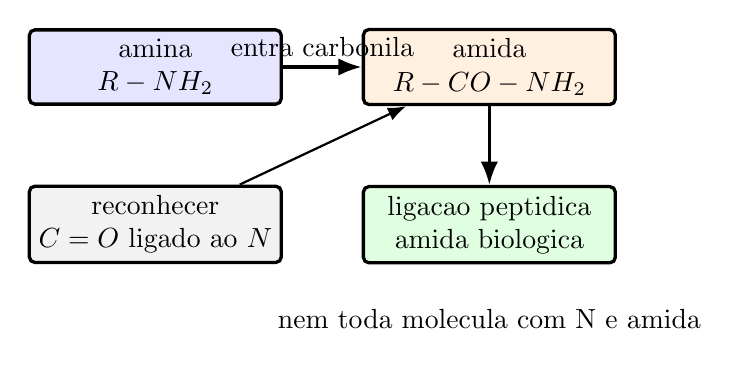
\begin{tikzpicture}[>=Latex,node distance=0.8cm]
  \tikzstyle{box}=[draw,rounded corners=2pt,very thick,minimum width=3.2cm,minimum height=0.85cm,align=center]
  \node[box,fill=blue!10] (amina) {amina\\$R-NH_2$};
  \node[box,fill=orange!12,right=1cm of amina] (amida) {amida\\$R-CO-NH_2$};
  \draw[very thick,->] (amina) -- (amida) node[midway,above] {entra carbonila};
  \node[box,fill=green!12,below=1cm of amida] (pep) {ligacao peptidica\\amida biologica};
  \draw[very thick,->] (amida) -- (pep);
  \node[box,fill=gray!10,below=1cm of amina] (crit) {reconhecer\\$C=O$ ligado ao $N$};
  \draw[thick,->] (crit) -- (amida);
  \node[align=center,below=0.45cm of pep] {nem toda molecula com N e amida};
\end{tikzpicture}
\end{document}
